\section{Introduction}
\label{s:intro}
The inverted pendulum is a control theory problem. The pendulum, which is freely hanging downwards, is attached to a cart\ (Figure \ref{fig:intro:initialpend}). The force can be applied to the cart, which moves it back and forth along the horizontal line. The applied force also, indirectly, moves the pendulum itself. The task is to apply the sequence of forces to a cart, which will swing the pendulum up\ (Figure \ref{fig:exps:swinguppend}) and keep it balanced in the upright position\ (Figure \ref{fig:exps:uprightpend}). In the double inverted pendulum, there is also an additional pendulum attached at the end of the first one.

\begin{figure}[!ht]
    \centering
    \begin{floatrow}
    \ffigbox[\FBwidth][\FBheight][t]{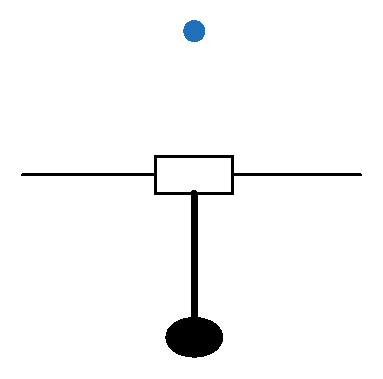
\includegraphics[width=0.3\textwidth,scale=0.4]{plots/initial_pendulum}}{\caption{The initial state: the pendulum is hanging downwards.}\label{fig:intro:initialpend}}
    \qquad
    \ffigbox[\FBwidth][\FBheight][t]{\includegraphics[width=0.3\textwidth,scale=0.4]{plots/swing_up_pendulum}}{\caption{The pendulum in the middle of the swing up action.}\label{fig:exps:swinguppend}}
    \qquad
    \ffigbox[\FBwidth][\FBheight][t]{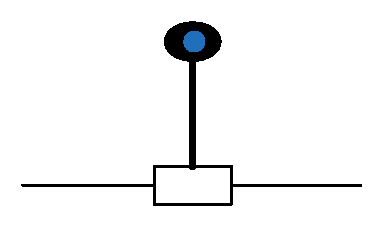
\includegraphics[width=0.3\textwidth,scale=0.4]{plots/upright_pendulum}}{\caption{The pendulum is in the upright position.}\label{fig:exps:uprightpend}}
    \end{floatrow}
\end{figure}

\noindent The task can be solved by deriving the controllers from the first principle\ (i.e., Lagrange's equations of motions). However, those controllers are task and parameters specific\ (e.g., different friction will result in a different controller). More general solution can be achieved if a controller is trained in reinforcement learning setting: an applied action is followed by a loss. The action is chosen to minimize the loss. There is only a single action in our problem, which is the force applied to a cart. The objective of the policy\ (i.e. controller) is the tip of the pendulum to be at the target: the upright position above the origin\ (the blue dot on the Figures \ref{fig:intro:initialpend}-\ref{fig:exps:uprightpend}). Thus, the loss is defined as the Euclidean distance between the tip of the pendulum and that target. 

\noindent The model-based reinforcement learning algorithm is used in this dissertation. First, the dynamics of the system is modeled solely from the data samples. The probabilistic model of the dynamics gives the predictions and its uncertainty on how the dynamical system evolves. Then, those information are used for the optimization of policy. The parameters of policy which give the predicted trajectory with the lower loss are preferable. The resulting policy is a closed-loop controller i.e. it uses information on current state for choosing next action.

\noindent The project aims to control a physical double inverted pendulum. The system is being recorded in real time using camera. The current state of the system is estimated from a frame, which introduces the noise and delay\ (the capture of frame and its transmission takes time) in observation. Basing on the estimated current state, the action is applied to the cart. Since the camera frame is a delayed version of the real state, the action itself is delayed. Finally, the velocities of the system are not directly observed from vision, which has implications to the representation of the system.

\noindent This dissertation is organized in the following order: the section \ref{s:pilco} describes the learning algorithm called \textit{PILCO}, probabilistic inference for control. It details how the dynamics and policy are being represented. It also outlines how both components are connected and trained; the section\ref{s:exps} presents the experiments with physical apparatus. It reports the results for single and double pendulum problems. The conclusions of this project can be found in the section \ref{s:con}.